% ===================== Who&When Pro =====================
\subsection{Who\&When Pro}\label{ds:who_and_when_pro}
\injected\ \okbadge\ \lbl{subset downloaded}\ \lbl{agent + step + failure mode}\ \lbl{single + multi-agent}\ \lbl{text / image / video}\ \lbl{26 benchmarks, 15 frameworks}

\begin{identity}
Paper & \emph{Who\&When Pro: Can LLMs Really Attribute Failures in AI Agents?} --- Liu, Xi, Zhang, Zeng, Yue, Wang, Kang, Wu, Wang (Penn State / AG2AI, Oregon State, Google DeepMind; the Who\&When group), ICML 2026, arXiv:2607.09996 \cite{whowhenpro2026}\\
Links & \href{https://huggingface.co/datasets/Leoxx/whowhen_pro}{HF \code{Leoxx/whowhen\_pro}} \textperiodcentered\ \href{https://github.com/ag2ai/whowhen_pro}{GitHub \code{ag2ai/whowhen\_pro}} (\code{whowhen\_eval} harness: per-framework renderers, LiteLLM runner, scorer, leaderboard; generation pipeline not yet released) \textperiodcentered\ \href{https://whowhenpro.github.io}{project page}\\
License & CC BY 4.0 (HF dataset card); upstream benchmark assets keep their own licences\\
Status & ungated; 21.7 GB in total (\code{text.jsonl} 75.6 MB, \code{video.jsonl} 21.3 MB, \code{image.jsonl} 6.79 GB, \code{image\_gui.jsonl} 11.19 GB with base64 screenshots, 21,850 video frames, \code{taxonomy.yaml}). \textbf{Subset downloaded}: text and video splits complete (6,257 + 916 rows), \code{taxonomy.yaml}, plus the first $\approx$1 GB of \code{image.jsonl} (166 rows) and of \code{image\_gui.jsonl} (118 rows); video frames not fetched; 1.36 GB in \code{data/who\_and\_when\_pro/}\\
\end{identity}

\begin{multicols}{2}
\paragraph{Description} The scaled-up successor of Who\&When: 12,326 failed trajectories of single- and multi-agent systems across text, image (incl.\ GUI) and video, with \emph{who} (agent), \emph{when} (step) and \emph{what} (error mode) labels that are exact \emph{by construction}. \textbf{Construction} (counterfactual replay + failure injection): base agents are run on each (framework, benchmark) pair and only \emph{successful} runs are kept as seeds. For a chosen step $t$ the successful prefix is replayed exactly (static tool calls from a SHA-256-keyed cache, stateful environments such as browsers, OSWorld and ALFWorld re-executed with fidelity checks), an erroneous action targeting one taxonomy mode is substituted at $t$---written by the base agent itself under an injection prompt, so it stays in-distribution---and the agent continues on-policy. Only continuations that end in failure are kept; traces that leak construction artefacts or where the answer is already salient before $t$ are filtered. Coverage: 26 benchmarks in 9 task categories, 15 frameworks:
\begin{itemize}
\item \textbf{text}: smolagents, MathChat, Magentic-One, Multi-Agent Debate, ALF-Agent (ReAct), MacNet, DyLAN, MetaGPT;
\item \textbf{image / GUI}: smolagents, PixelCraft, Debate; CoAct-1, OpenAI-CUA, AgentOccam, Gemini/WebVoyager;
\item \textbf{video}: EVA, DVD (LVBench).
\end{itemize}
7 of the 15 frameworks are single-agent. \textbf{Taxonomy}: six families---Perception (P.1--2), Reasoning (R.1 hallucination, R.2 reasoning, R.3 numerical, R.4 task misunderstanding), Planning (PL.1--2), Action (A.1 tool parameter, A.2 output format, A.3 premature termination, A.4 looping), Verification (V.1 context loss, V.2 inadequate verification), Coordination (C.1 delegation, C.2 communication, C.3 over-reliance); the paper says 18 modes, the released \code{taxonomy.yaml} has 17. \textbf{Validation}: three author-side annotators reviewed 100 stratified traces: 94\% of step and 90\% of agent/family labels approved, Fleiss' $\kappa$ = 0.73, 2\% judged to have no clear decisive error.

\paragraph{Metrics and baselines} Predict agent (scored on multi-agent traces only), step coordinate (exact match; Step@$k$ tolerance in the appendix) and error mode (macro-F1); \emph{Joint} = all three correct; per-framework averages. Protocols: All-at-Once, Step-by-Step, Binary-Search. All-at-Once, Agent / Step / Error / Joint in \% (paper):

\begin{center}\footnotesize
\begin{tabular}{@{}llrrrr@{}}\toprule
Model & Split & Agent & Step & Error & Joint\\\midrule
GPT-5.4 & text & \textbf{55.7} & \textbf{72.3} & 15.3 & 21.3\\
Claude Sonnet 4.6 & text & 54.9 & 69.8 & \textbf{19.1} & \textbf{22.4}\\
Gemini 3 Flash & text & 52.1 & 71.2 & 16.2 & 17.3\\\midrule
GPT-5.4 & image & \textbf{67.7} & \textbf{65.2} & 26.5 & \textbf{30.2}\\
Claude Sonnet 4.6 & image & 67.5 & 63.8 & \textbf{29.5} & 29.6\\
Gemini 3 Flash & image & 62.5 & 63.9 & 26.0 & 29.6\\\midrule
GPT-5.4 & video & \textbf{85.1} & 60.5 & 33.8 & 21.6\\
Claude Sonnet 4.6 & video & 79.8 & \textbf{64.4} & 37.4 & \textbf{26.4}\\
Gemini 3 Flash & video & 74.4 & 59.8 & \textbf{40.0} & 23.0\\\bottomrule
\end{tabular}
\end{center}
Best open-weight text results: Qwen3.5-122B Step 73.9, GLM-5 Joint 25.3. Step@1 tolerance adds +13.9 pp (text), +16.9 (image), +28.1 (video). Headline finding: models detect \emph{symptoms} but mis-locate \emph{root causes} (low Error/Joint), worst on multimodal and long traces.

\paragraph{Schema} \code{data/<split>.jsonl}, one row per trace: \code{id} (\code{<benchmark>\_<framework>\_<nnnn>}), \code{framework}, \code{benchmark}, and JSON-encoded strings \code{task} (\{\code{query}, \code{answer}, \code{options?}, \code{images?}\}), \code{trajectory}, \code{ground\_truth} (\{\code{mode}, \code{agent}\,|\,\code{agents}, \code{step}\,|\,\code{round}+\code{position}\,|\,\code{stage}, \code{accepted\_predictions?}\}; \code{agent} is \code{null} for single-agent frameworks) and \code{extras} (agent roster, \code{final\_answer}, \code{termination}, \code{topology}, \code{post\_injection\_turns}, \ldots). The \code{trajectory} shape is \emph{framework-specific}---8 shapes and 5 step-coordinate conventions: flat 1-based \code{step\_number} (ALF-Agent, GUI agents), flat cursor starting at 0 if a planning step exists (smolagents), \code{"R.P"} round.position with P\,=\,0 orchestrator / 1 specialist (Magentic-One; round-only for Debate/DyLAN), \code{stage} 0/1/2 (MetaGPT, MacNet) and native index minus an offset (DVD/EVA). Injected and replayed entries are flagged in the raw rows (\code{is\_injected}, \code{injected}, \code{phase}, \code{is\_replayed}); the official renderers strip them.
\end{multicols}

\paragraph{Statistics} computed from the downloaded subset (7,457 of 12,326 rows: text and video complete; image and image\_gui are the first rows of each file, i.e.\ browsecomp\_vl/smolagents and webvoyager/AgentOccam + 2 OSWorld/CoAct rows---indicative only).\par\nobreak\vspace{1pt}
\noindent\begin{minipage}[t]{0.60\linewidth}\vspace{0pt}\small
{\footnotesize\setlength{\tabcolsep}{3.5pt}\begin{tabular}{@{}lrrrrr@{}}\toprule
 & All & text & video & image$^\ast$ & image\_gui$^\ast$\\\midrule
trajectories (all failed, one injection) & 7457 & 6257 & 916 & 166 & 118\\
scorable steps: mean / median & 5.7 / 4 & 6.1 / 4 & 3.1 / 2 & 3.8 / 4 & 7.1 / 4\\
steps: min -- max & 1 -- 79 & 1 -- 31 & 2 -- 49 & 1 -- 12 & 1 -- 79\\
injected step rel.\ pos.: mean / median & 0.74 / 0.83 & 0.73 / 0.80 & 0.79 / 1.0 & 0.84 / 1.0 & 0.56 / 0.50\\
characters / traj.\ (no images): mean & 9.4\,k & 8.6\,k & 15.4\,k & 9.0\,k & 6.4\,k\\
characters / traj.: median & 4.7\,k & 5.1\,k & 1.3\,k & 8.3\,k & 3.0\,k\\\bottomrule
\end{tabular}}

\smallskip Roster size mean 1.9 (max 5); 4,617 single-agent vs 2,840 multi-agent rows (62\% / 38\%); 0 rows whose label could not be matched to a rendered step. 12 of the 15 frameworks and 20 of the 26 benchmarks appear in the subset---rows per framework: smolagents 3,442, MathChat 920, Magentic-One 811, EVA 748, Debate 445, ALF-Agent 311, MacNet 261, DVD 168, DyLAN 152, AgentOccam 116, MetaGPT 81, CoAct 2. Several frameworks have fixed lengths: Debate always 6 steps (2 rounds $\times$ 3 agents), MacNet 4, MetaGPT 3, ALF-Agent always 30 (the step budget); smolagents 4.5 and Magentic-One 6.1 on average. Error families: R 59\%, A 22\%, V 9\%, C 5\%, P 3\%, PL 2\%. Faulty agent on multi-agent rows is nearly constant per framework: MathChat \code{assistant} 100\%, Magentic-One \code{orchestrator} 78\%, MetaGPT \code{architect} 83\%, DVD \code{orchestrator} 90\%; Debate/DyLAN labels list several agents (C.3 over-reliance).
\end{minipage}\hfill
\begin{minipage}[t]{0.38\linewidth}\vspace{0pt}
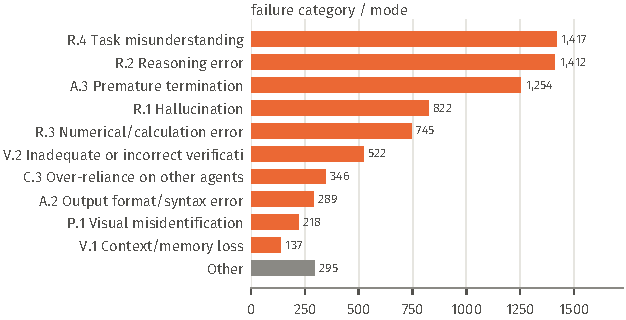
\includegraphics[width=\linewidth]{figures/cat_who_and_when_pro.pdf}
\end{minipage}

\paragraph{Example trajectory} Row \code{gaia\_magentic-one\_0044} (text split; 7 scorable steps, 5-agent roster, 1.9\,k characters). The injected WebSurfer step 0.1 (a Bing search) is labelled a hallucination; from there the orchestrator works with 791.8\,k women and 586.9\,k men, and Coder and ComputerTerminal faithfully compute 204.9 (ground truth 234.9). Label: \code{websurfer}, step \code{"0.1"}, mode R.1 (hallucination); no free-text reason exists.
% auto-generated by scripts/render_traj.py -- do not edit
\trajtask{gaia\_magentic-one\_0044}{Take the gender split from the 2011 Bulgarian census about those who have completed tertiary education. Subtract the smaller number from the larger number,\allowbreak{} then return the difference in thousands of women. So if there were 30.1 thousand more men,\allowbreak{} you'd give "30.1"\par Provide a concise,\allowbreak{} precise answer. State your final answer on the last line,\allowbreak{} prefixed with "FINAL ANSWER:\allowbreak{} "}
\begin{trajstep}{0.0}{orchestrator}{agA}
Search for the official 2011 Bulgarian census data on educational attainment,\allowbreak{} specifically the number of men and women who have completed tertiary education. Extract the relevant numbers.
\end{trajstep}
\begin{faultystep}{0.1}{websurfer}{agB}
I typed '2011 POPULATION CENSUS Main Results tertiary education men women 2011 Bulgaria' into the search bar.\newline The web browser is open to the page [2011 Bulgarian census educational attainment tertiary education numbers by gender - Search](https:\allowbreak{}/\allowbreak{}/\allowbreak{}www.bing.com/\allowbreak{}search?\allowbreak{}q=\allowbreak{}2011+Bulgarian+census+educational+attainment+tertiary+education+numbers+by+gender\&form=\allowbreak{}QBLH\&sp=\allowbreak{}-1\&lq=\allowbreak{}0\&pq=\allowbreak{}\&sc=\allowbreak{}0-0\&qs=\allowbreak{}n\&sk=\allowbreak{}\&cvid=\allowbreak{}0A81DC5DB135488789B8CEA69382C803).\newline The viewport shows 54\% of the webpage.\newline The following text is visible in the viewport:\allowbreak{}\newline - ``[PDF] 2011 POPULATION CENSUS Main Results - nsi.bg''\newline - ``Women have completed tertiary education significantly more oft\newline [...] (245 chars omitted) [...]\newline attainment and extract the number of men and women with tertiary education,\allowbreak{} I will enter a relevant query into the search box.",\allowbreak{} "input\_field\_id":\allowbreak{} 59,\allowbreak{} "text\_value":\allowbreak{} "2011 Bulgarian census educational attainment tertiary education numbers by gender"\}\}]
\end{faultystep}
\begin{trajstep}{1.0}{orchestrator}{agA}
Subtract 586.9 from 791.8 to get the difference in thousands of women who completed tertiary education according to the 2011 Bulgarian census. Output the answer as:\allowbreak{} 'FINAL ANSWER:\allowbreak{} [number]'
\end{trajstep}
\begin{trajstep}{1.1}{coder}{agC}
```python\newline women =\allowbreak{} 791.8\newline men =\allowbreak{} 586.9\newline difference =\allowbreak{} women - men\newline print(f"FINAL ANSWER:\allowbreak{} \{difference:\allowbreak{}.1f\}")\newline ```
\end{trajstep}
\begin{trajstep}{2.0}{orchestrator}{agA}
Run the provided Python code to output the final answer.
\end{trajstep}
\begin{trajstep}{2.1}{computerterminal}{agD}
FINAL ANSWER:\allowbreak{} 204.9
\end{trajstep}
\begin{trajstep}{3.0}{orchestrator}{agA}
According to the 2011 Bulgarian census,\allowbreak{} 791.8 thousand women and 586.9 thousand men had completed tertiary education. The difference between these numbers is 204.9 thousand,\allowbreak{} with more women than men.\par FINAL ANSWER:\allowbreak{} 204.9
\end{trajstep}
\trajannotation{websurfer}{0.1}{R.1 (Hallucination)}{}{234.9}{204.9}{\textbf{ground\_truth\_raw}: \{"agent":\allowbreak{} "websurfer",\allowbreak{} "step":\allowbreak{} "0.1",\allowbreak{} "mode":\allowbreak{} "R.1"\}; \textbf{framework}: magentic-one; \textbf{benchmark}: gaia; \textbf{extras}: \{"agents":\allowbreak{} [\{"id":\allowbreak{} "orchestrator",\allowbreak{} "role":\allowbreak{} "Orchestrator"\},\allowbreak{} \{"id":\allowbreak{} "websurfer",\allowbreak{} "role":\allowbreak{} "WebSurfer"\},\allowbreak{} \{"id":\allowbreak{} "coder",\allowbreak{} "role":\allowbreak{} "Coder"\},\allowbreak{} \{"id":\allowbreak{} "filesurfer",\allowbreak{} "role":\allowbreak{} "FileSurfer"\},\allowbreak{} \{"id":\allowbreak{} "computerterminal",\allowbreak{} "role":\allowbreak{} "ComputerTerminal"\}],\allowbreak{} "final\_answer":\allowbreak{} "204.9",\allowbreak{} "termination":\allowbreak{} "satisfied"\}; \textbf{step\_indexing}: framework-specific coordinate as rendered by the official harness (see script docstring); \textbf{injected\_entries}: [2]}


\paragraph{Notes} (i) Labels by construction, not annotation: exact (agent, step, mode) and no rationale, but the failures are synthetic and on-policy-but-prompted. Because the replayed prefix must be a correct prefix of a successful run, injections sit late (mean relative position 0.74, median 0.83; paper: 64\% in the 40--80\% range) whereas natural-failure datasets put the decisive error near the middle (Who\&When 0.46, TraceElephant 0.47, MP-Bench 0.40). (ii) Mostly single-agent and short: 62\% of rows have one agent, median length is 4 steps, and the agent axis is scored only on the 38\% multi-agent rows where the culprit is often predictable from the framework alone. Only Magentic-One (GAIA, SimpleQA-Verified) resembles the Who\&When / TraceElephant / MP-Bench setting. (iii) No common step format: the harness's renderers and scorer must be reproduced exactly for comparable numbers (our statistics follow them); Debate/DyLAN are scored at round level and 109 MacNet rows carry \code{accepted\_predictions} alternates---even this benchmark concedes multiple acceptable answers. (iv) Label leakage: injected/replayed flags inside \code{trajectory} must be stripped before evaluation. (v) Taxonomy: paper 18 modes vs.\ 17 in \code{taxonomy.yaml} with slightly different names; Reasoning + Action modes make up 81\% of labels, Coordination 5\%, Perception/Planning are rare in the text split. (vi) Practical: text + video (97 MB) suffice for text-only attribution experiments; image/GUI rows embed screenshots (18 GB); an earlier anonymous release \code{tmpxv7/who-when-pro} (18-mode taxonomy) and a text-only re-upload also circulate.
